\section{Gleichstromnetzwerke}

\subsection{Pfeilsysteme}
\begin{multicols}{2}
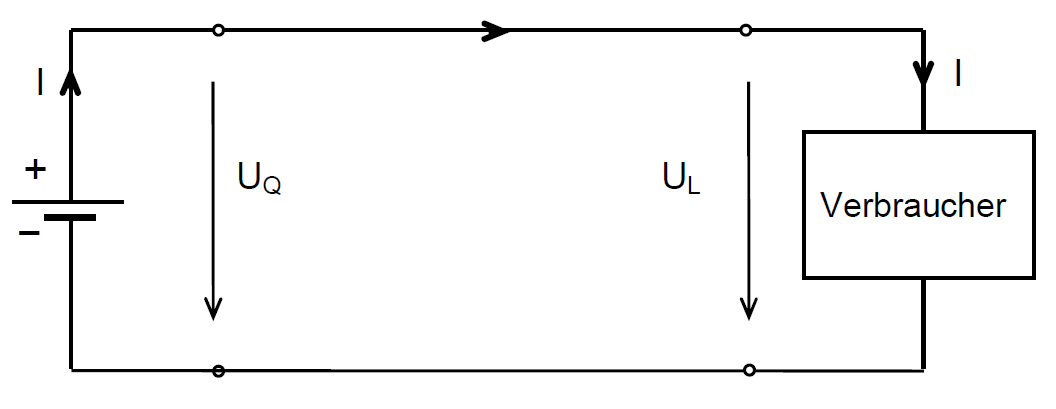
\includegraphics[width=0.50\textwidth]{pics/dcnet/pfeilsysteme}\\
\begin{itemize}
	\item Erzeuger-Pfeilsystem: Spannungs- und Strompfeil \textbf{entgegengesetzt}\\
	\item Verbraucher-Pfeilsystem: \textbf{gleiche} Bezugsrichtung f"ur Strom und Spannung\\
\end{itemize}
\end{multicols}
\begin{multicols}{2}
\subsection{lineare Widerst"ande}
$U=R \cdot I \rightarrow \lbrack V = \Omega  \cdot  A \rbrack$ \\

\subsection{Leistung an linearen Widerst"ande}
$P=U \cdot I \ \rightarrow P=R \cdot I^2 = \frac{U^2}{R}$

\subsection{Nonlineare Widerst"ande}
Als differenzielle Widerst"ande bezeichnet man die Steigung der Tangente an einem bestimmten Punkt.\\
$r = \frac{\Delta U}{\Delta I}$\\

\subsection{Spezifischer Widerstand und Leitf"ahigkeit}
$R=\frac{\rho \mathit{l}}{A}=\frac{\mathit{l}}{\sigma \cdot A}$ $\rightarrow$ $\lbrack \rho \rbrack = \frac{ \Omega \cdot mm^2}{m}$,$\lbrack \sigma \rbrack = \frac{1}{\rho}$,$ \lbrack \mathit{l} \rbrack = m$

\subsection{Temperaturabh"anigkeit von Widerst"anden}
\begin{itemize}
	\item PTC: Kaltleiter, temp. hoch $\rightarrow$ Widerstand hoch
	\item NTC: Warmleiter, temp. hoch $\rightarrow$ Widerstand tief
\end{itemize}
$\Delta R = R_{20} \cdot \alpha_{20} \cdot \Delta \vartheta$ $\rightarrow$ $R = R_{20} \cdot (1 + \alpha_{20} \cdot \Delta \vartheta)$\\
$\alpha$ = Temperaturkoeffizient, $\alpha_{20}=\frac{\Delta R}{ R_{20} \cdot \Delta \vartheta} \rightarrow \lbrack \frac{1}{K} \rbrack$\\
0°C = 273,15K

\end{multicols}

\subsection{Ideale Spannungsquellen}
\begin{multicols}{4}
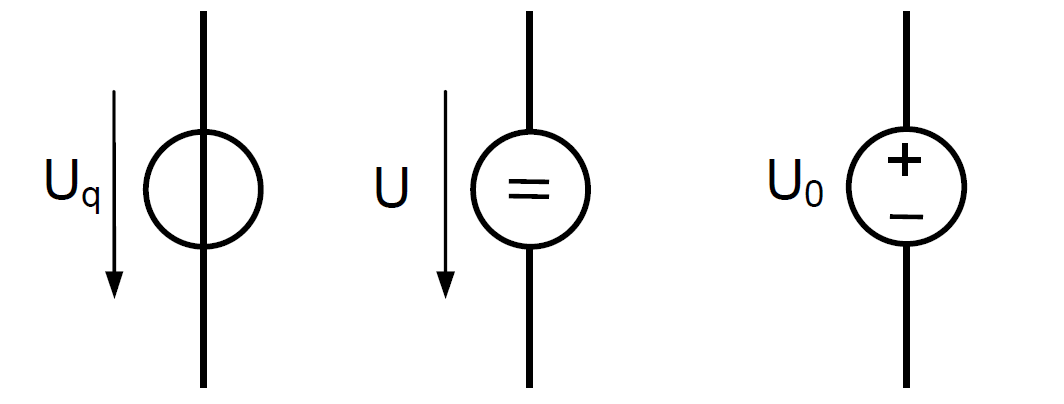
\includegraphics[width=0.25\textwidth]{pics/quellen/UQsymbole}\\
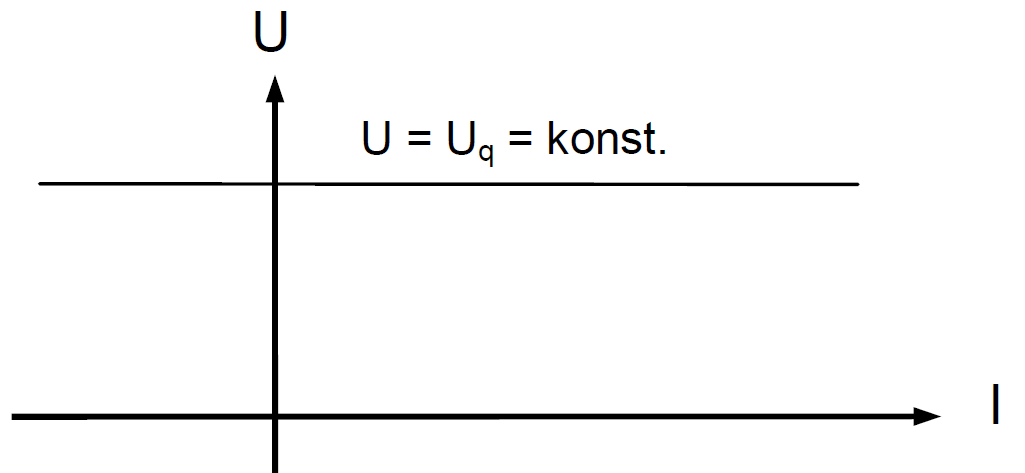
\includegraphics[width=0.25\textwidth]{pics/quellen/QUkennlinie}\\
Der Strom h"angt von der Last an der Spannungsquelle ab.\\
\end{multicols}

\subsection{Lineare Spannungsquellen}
\begin{multicols}{4}
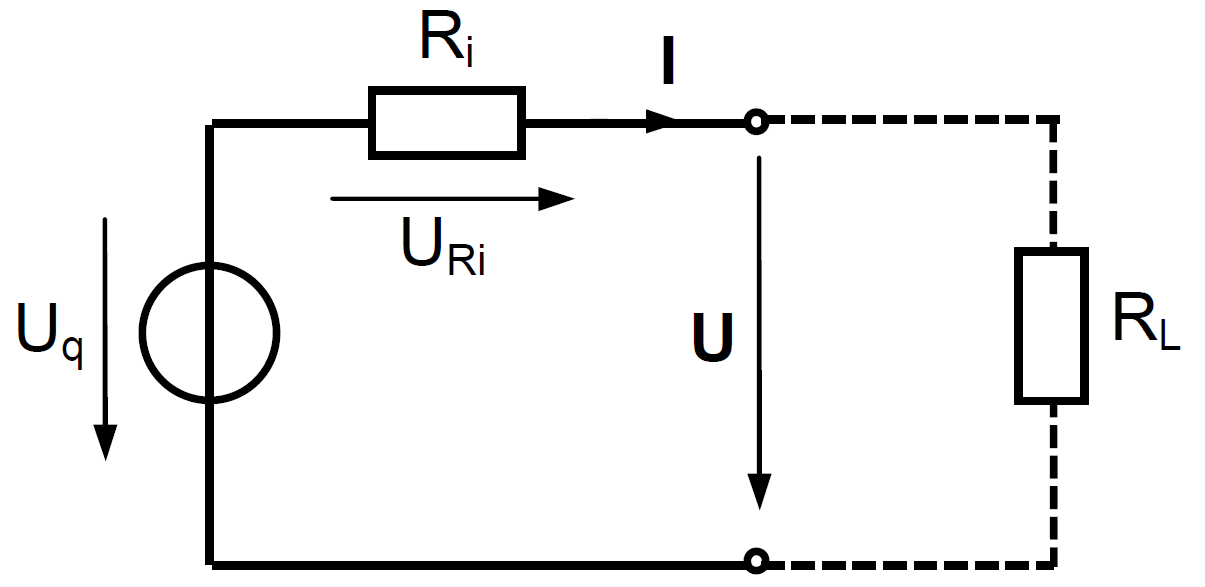
\includegraphics[width=0.25\textwidth]{pics/quellen/lUEquelle}\\
$U_q\ =$ Leerlaufspannung
$U\ =$ Klemmenspannung
$R_I\ =$Innenwiderstand
$R_I=\frac{U_q}{I_K}$\\
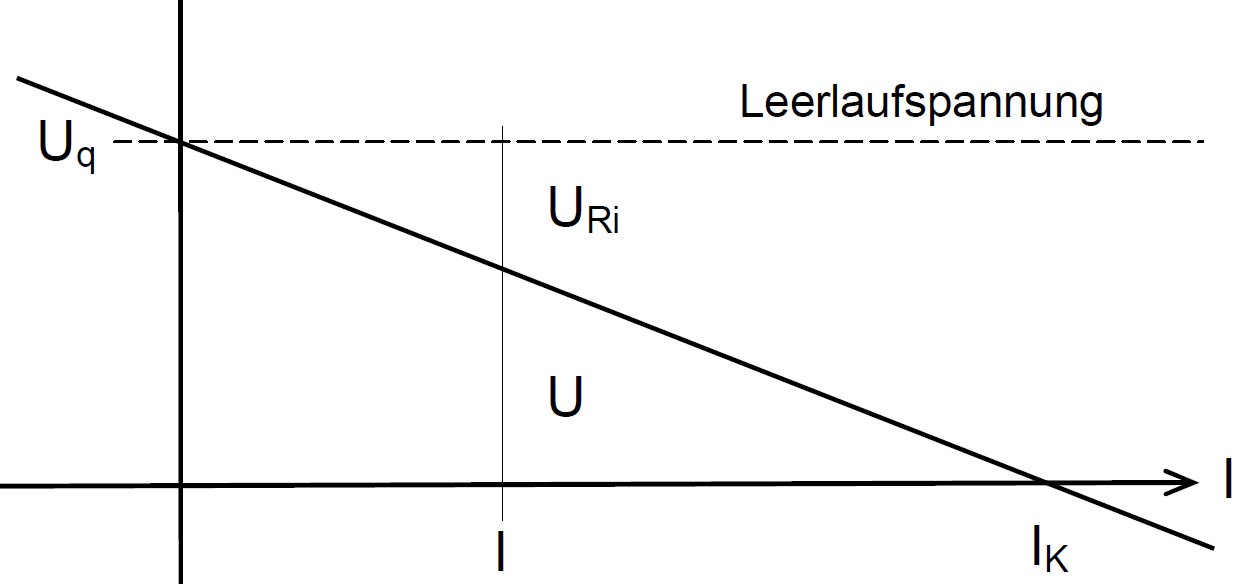
\includegraphics[width=0.25\textwidth]{pics/quellen/UIkennlinie}\\
$I_K\ =$Kurzschlussstrom $(U=0)$\\
\end{multicols}

\subsection{Ideale Stromquellen}
\begin{multicols}{4}
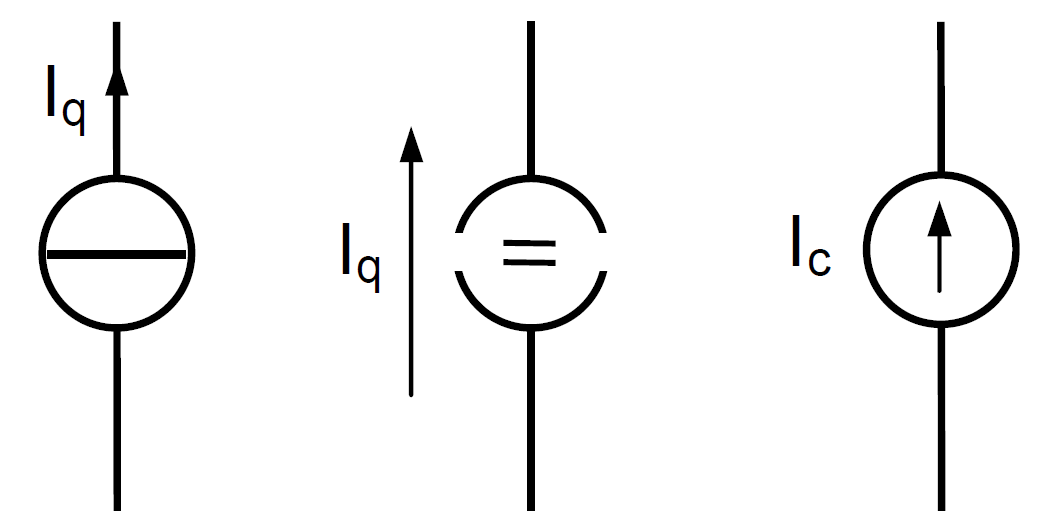
\includegraphics[width=0.25\textwidth]{pics/quellen/IQsymbole}\\
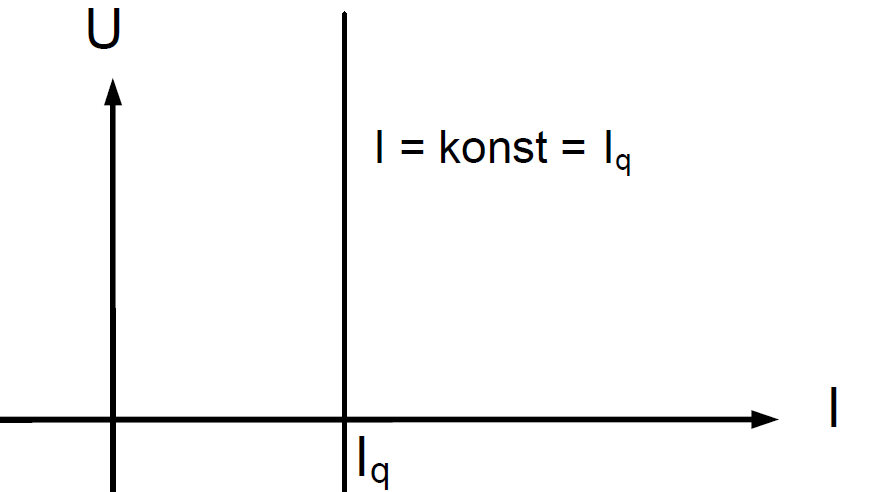
\includegraphics[width=0.25\textwidth]{pics/quellen/QIkennlinie}\\
Wird eine Quelle kurzgeschlossen ($R_L = 0$), so ist die Klemmenspannung $U=0$\\
\end{multicols}

\subsection{Lineare Quellen}
\begin{multicols}{4}
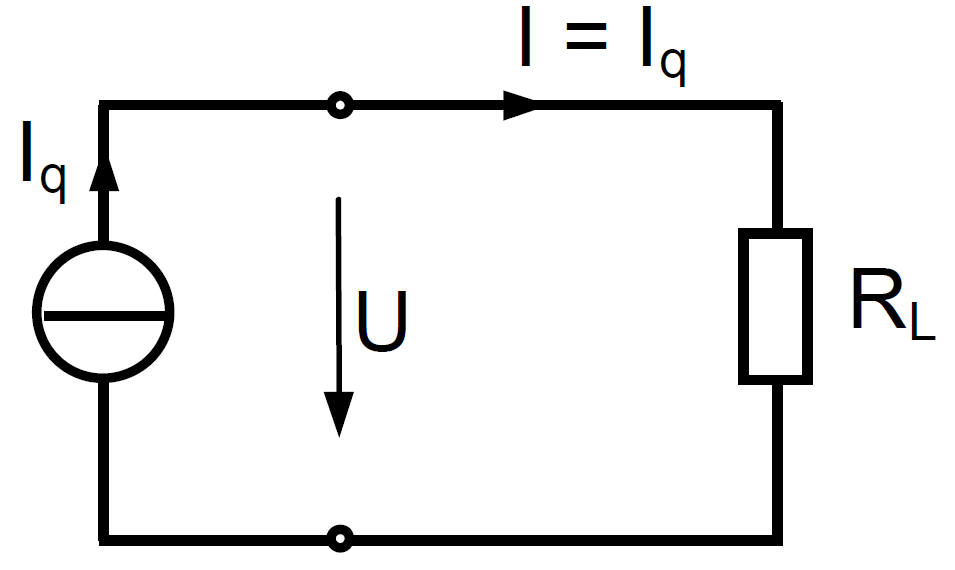
\includegraphics[width=0.25\textwidth]{pics/quellen/lIEquellen}\\
$R_i=\frac{U_0}{I_q}=\frac{U_0}{I_K}=\frac{Leerlaufspannung}{Kurzschlussstrom}$\\
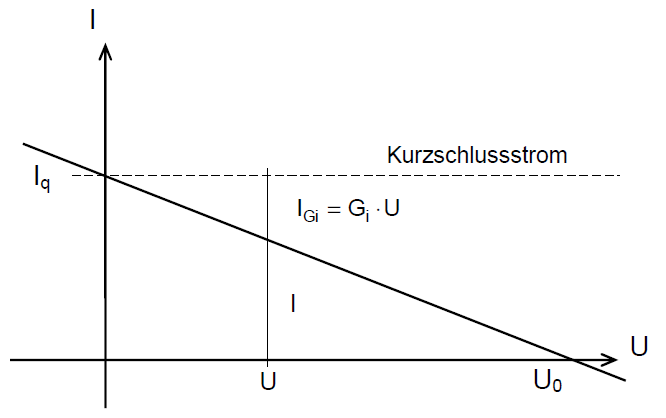
\includegraphics[width=0.25\textwidth]{pics/quellen/IUkennlinie}\\
$U_0=$Leerlaufspannung ($I=0!$)\\

\end{multicols}

\begin{multicols}{3}
Spannungsquelle nach Thévenin\\
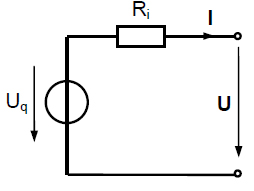
\includegraphics[width=0.2\textwidth]{pics/dcnet/ersatz_spannung}\\
Stromquelle nach Norton\\
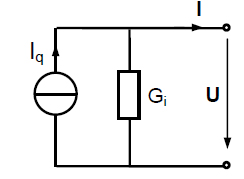
\includegraphics[width=0.2\textwidth]{pics/dcnet/ersatz_strom}\\
Formeln\\
$ U_q = U_0 $\\
$ R_i = \frac{U_q}{I_K} = \frac{U_0}{I_K} $\\
$ G_i = \frac{I_K}{U_0}\ \ \ \ \ R_i = \frac{1}{G_i}$\\
$ I_q = I_K $\\
Umwandlung: Ri ist bei beiden gleich!
\end{multicols}

\subsection{Lineare Quellen - nonlinearer Widerstand}
\begin{multicols}{2}
\begin{itemize}
\item Gegeben: $U_q$, $R_I$ von linearer Quelle Kennlinie von nichtlinearem Widerstand
\item Gesucht: Klemenstannung $U$ und Strom $(I = I_Q = I_L)$
\item Vorgehen: I-U-Kennlinie von beiden Zweipolen in dasselbe Diagramm eintragen:
\end{itemize}
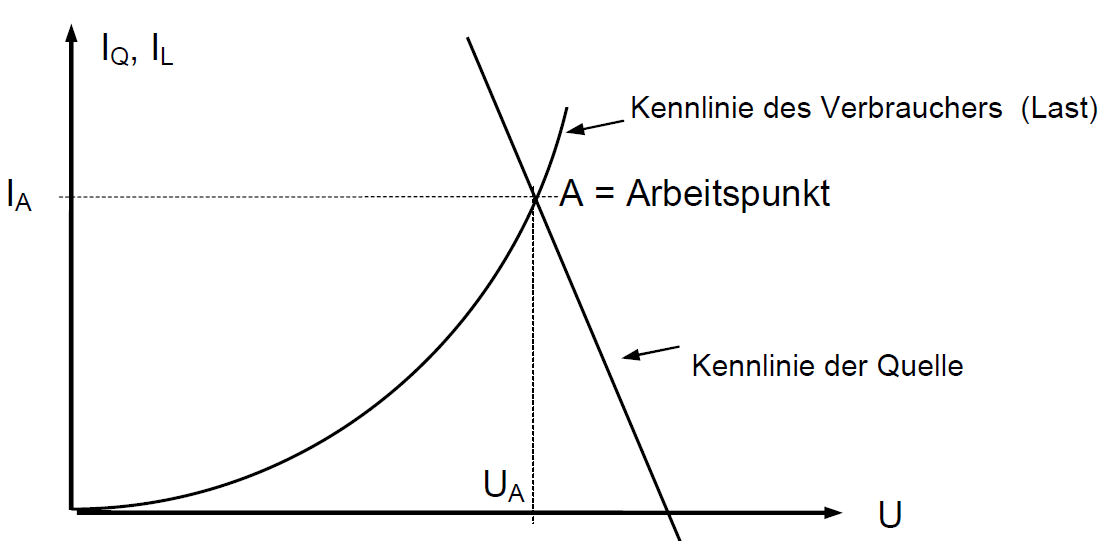
\includegraphics[width=0.3\textwidth]{pics/quellen/nonlineUI}
\end{multicols}

\subsection{Addition von nonlinearen Zweipolen}
\begin{multicols}{2}
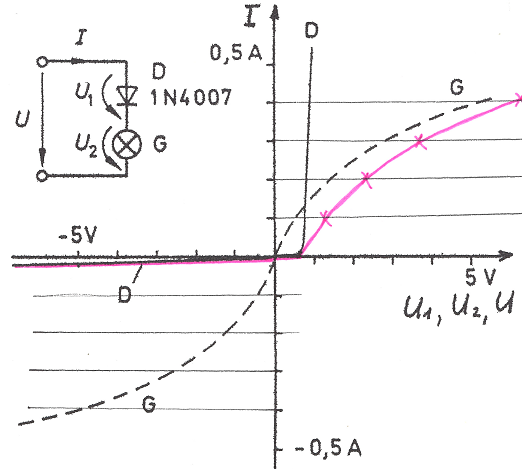
\includegraphics[width=0.3\textwidth]{pics/kennlinien/nonlinAddPar}\\
Serieschaltung: Teilspannungen bei gleichen Str"omen addieren.\\
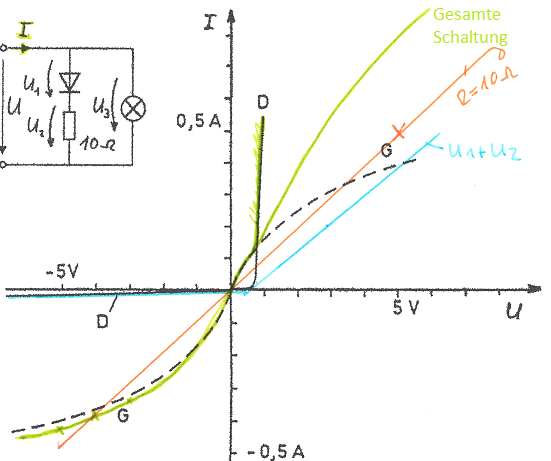
\includegraphics[width=0.3\textwidth]{pics/kennlinien/nonlinAddSer}\\
Parallelschaltung: Str"ome bei gleicher Spannung addieren.\\
\end{multicols}

\subsection{Wirkungsgrad}
\begin{tabular}{ll}
Wirkungsgrad & $n = \frac{P_{ab}}{P_{zu}}$ \\
& $ P_{zu} = P_{ab}+P_{verlust} $\\
& $ n_{tot} = n_1 \cdot n_2 \cdot n_3 $\\
Bei realen Quellen & $n = \frac{abgegebene Leistung}{abgeg. Leistung + innere Verlustleistung}$\\
Bei lin. U-Quelle & Innere Verluste bei Leerlauf = 0\\
& Bei Kurzschluss Max-Wert $P_{max} = R_i \cdot I_k^2$\\
Bei lin. I-Quelle & Innere Verluste bei Kurzschluss = 0\\
& Bei Leerlauf Max-Wert $P_{max} = G_i \cdot U_0^2$\\
\end{tabular}\\
Vorsicht: Obwohl die Schaltungen äquivalent sind, sind die inneren Verluste NICHT gleich!

\subsection{Leistungsanpassung}
$R_i = R_L$ \\
$P_{max} = \frac{U_q^2}{4 \cdot R_i} = \frac{I_q^2}{4 \cdot G_i}$\\
n beträgt 50\%; am $R_i$ wird gleich grosse P umgesetzt wie am $R_L$\\

\subsection{Wheatstone Brücken}
\subsubsection{Anwendung}
\begin{itemize}
\item Messungen von Widerständen (bei Wechselstrom: auch Bestimmung von L, C samt Verlustfaktor)
\item In Verbindung mit Sensoren (Temp.- oder Druckabhängige Widerstände: Bestimmung von Temp, Kraft, etc.)
\end{itemize}
\subsubsection{Speisung mit U-Quellen}
\begin{tabular}{lll}
Abgeglichene & Nicht abgeglichene & Mit $R_L$ belastet \\
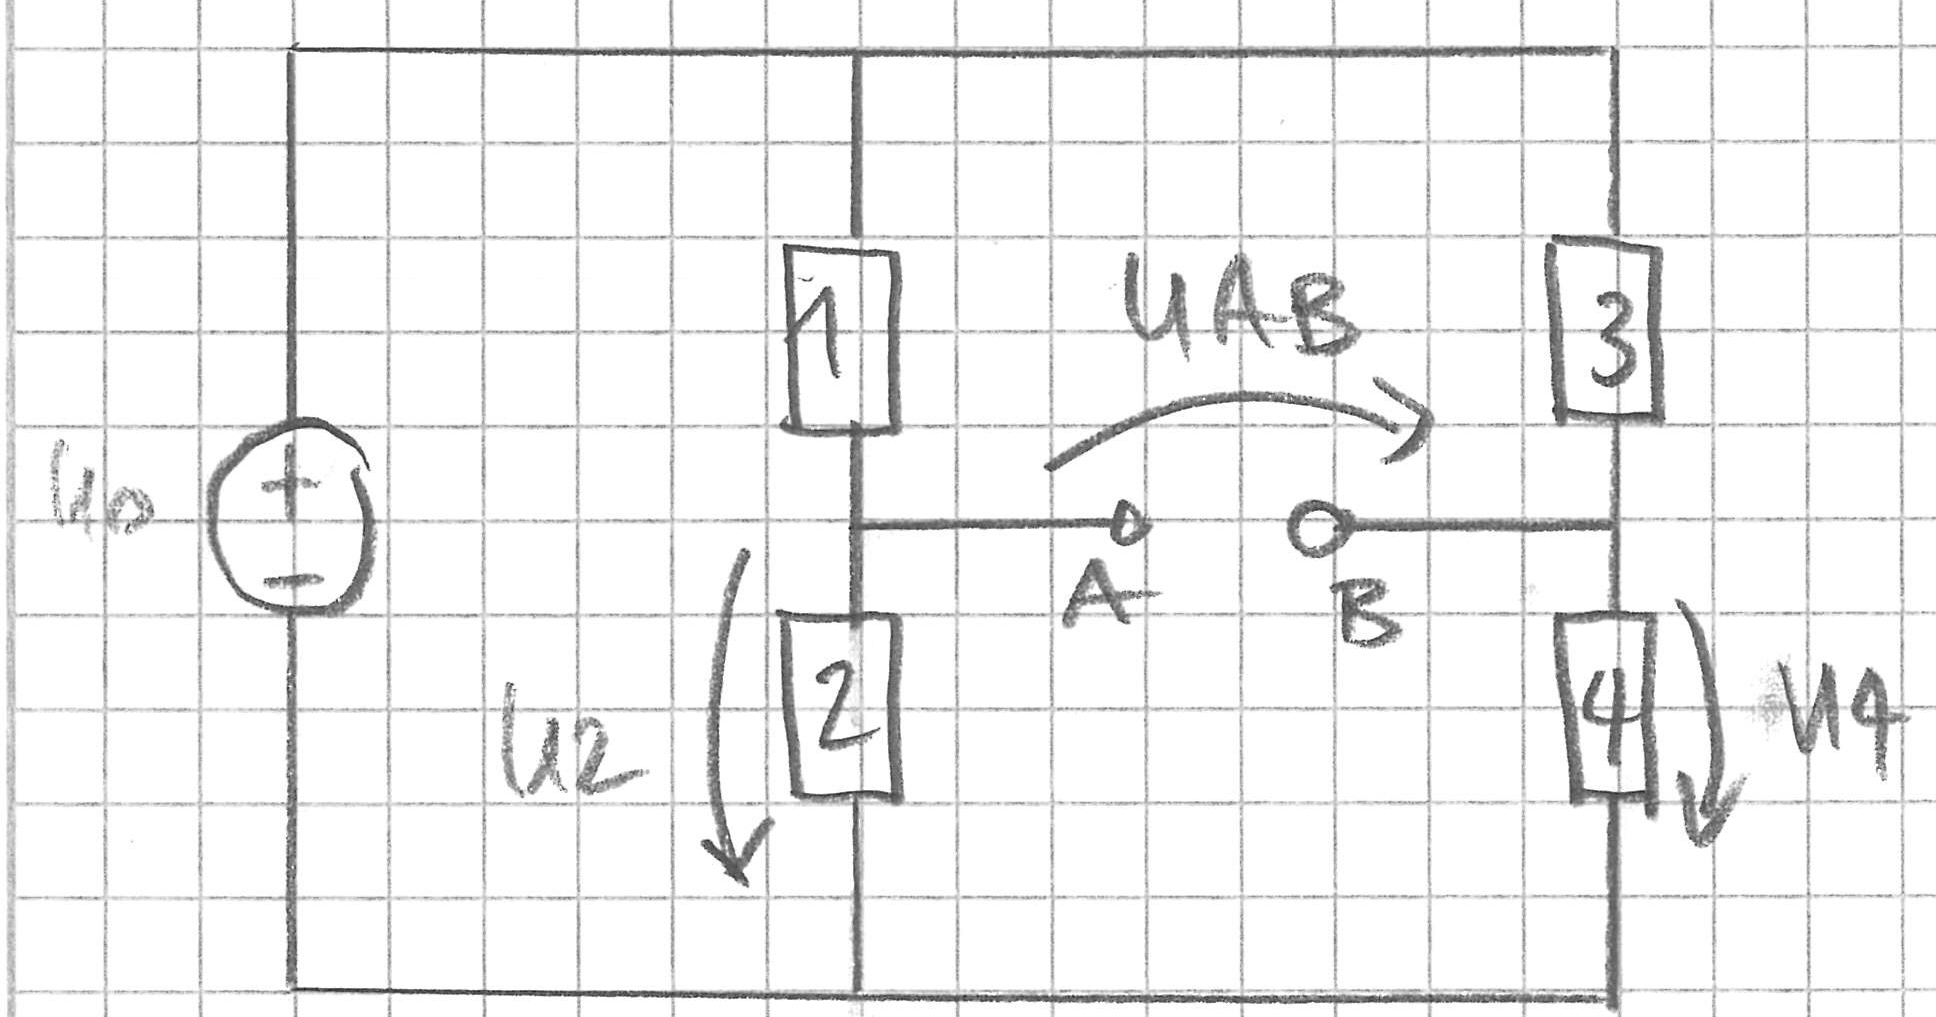
\includegraphics[width=0.3\textwidth]{pics/wheatstone/u_quelle_abgeglichen} & 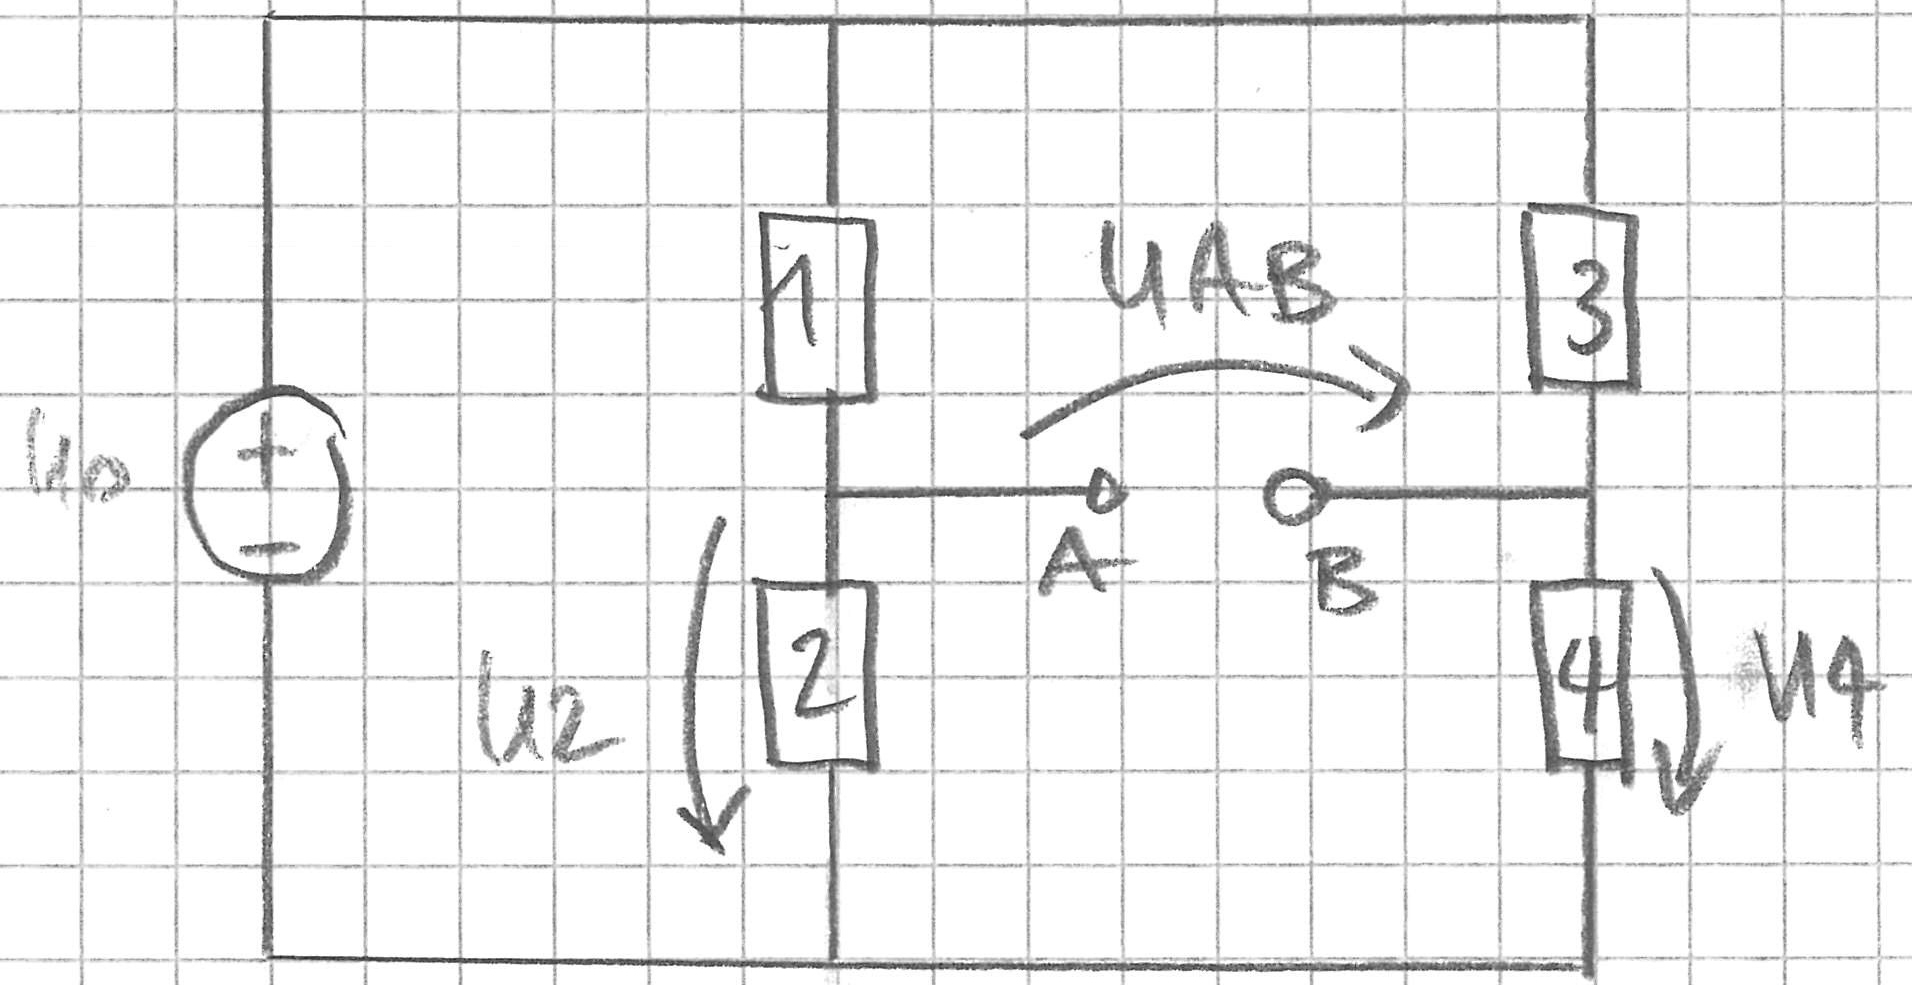
\includegraphics[width=0.3\textwidth]{pics/wheatstone/u_quelle_nicht_abgeglichen} & 
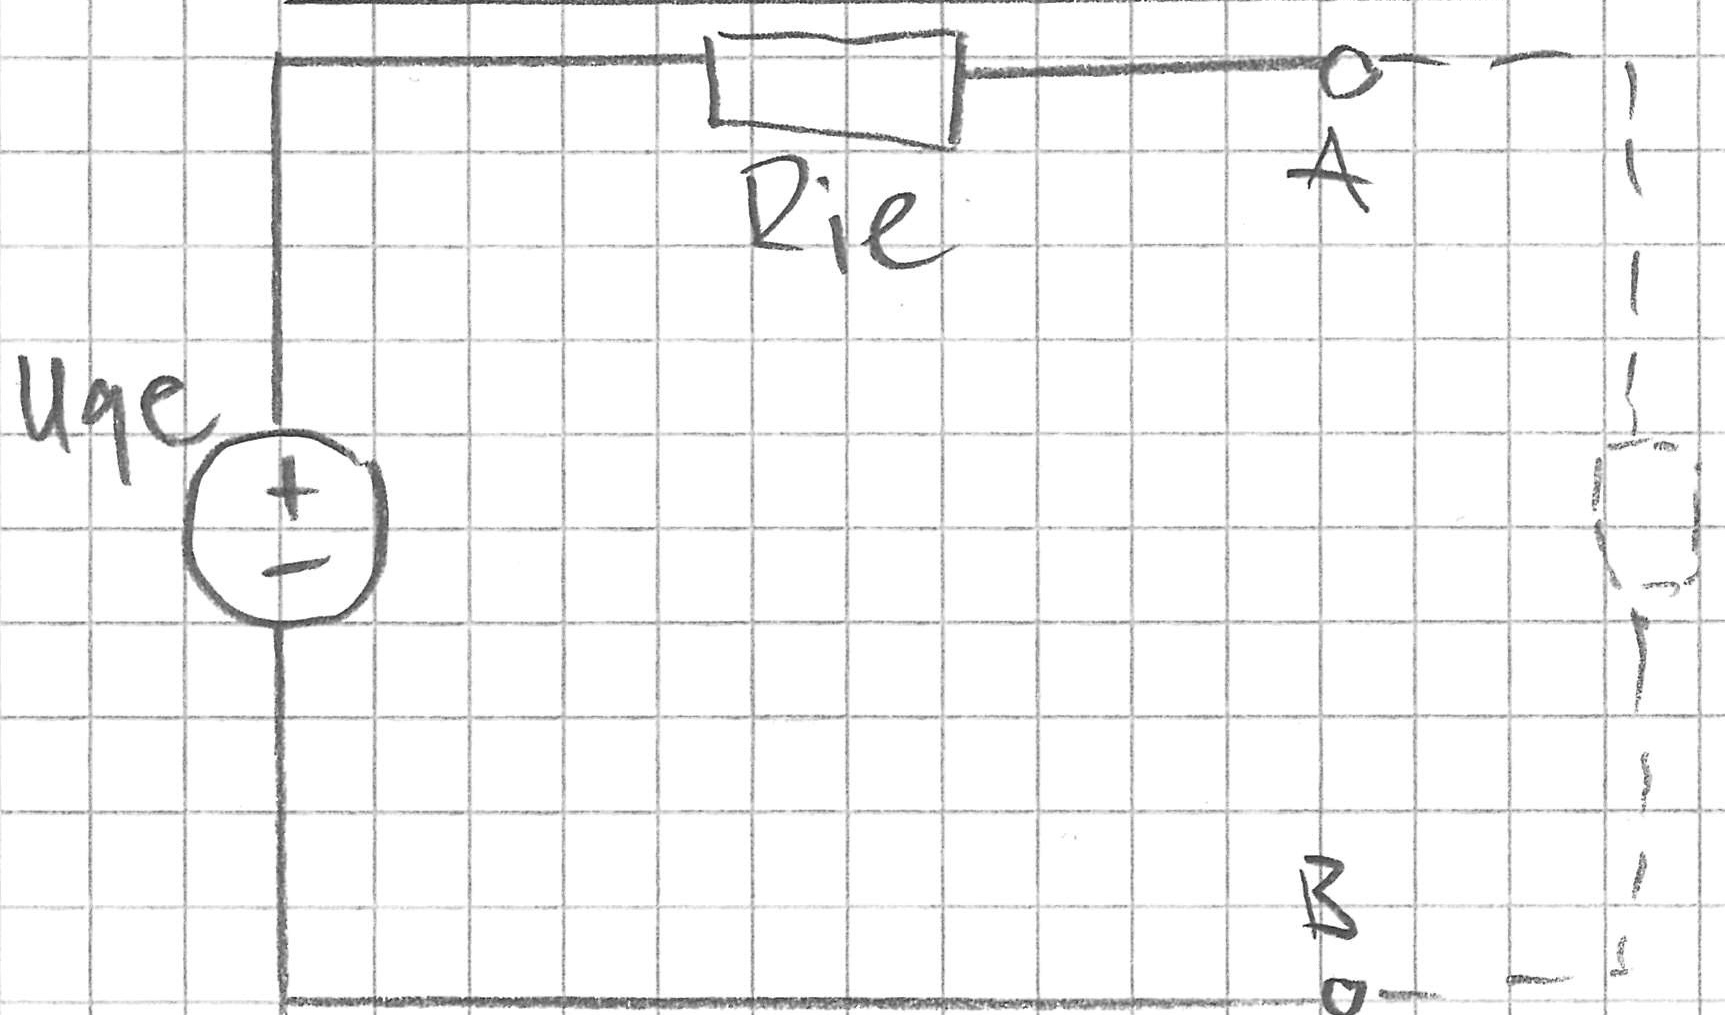
\includegraphics[width=0.25\textwidth]{pics/wheatstone/belastet} \\
$U_{AB} = Brueckenspannung$ & A-B offen: & $U_{AB} = U_{qe} \cdot
\frac{R_L}{R_{ie} + R_L}$ \\ abgeglichen falls $U_{AB} = 0$ & $U_{AB} = U_2 - U_4$ & \\
d.h. $ U_2 = U_4 $ & $U_{AB} = U_0(\frac{R_2}{R_1 + R_2} - \frac{R_4}{R_3 + R_4})$ & \\
Abgleichbedingung: $ \frac{R_1}{R_2} = \frac{R_3}{R_4 } $ &  $ U_{BA} = U_0(\frac{R_4}{R_3+R_4} - \frac{R_2}{R_1+R_2})$& \\
\end{tabular}

\subsubsection{Speisung mit I-Quellen}
\begin{tabular}{ll}
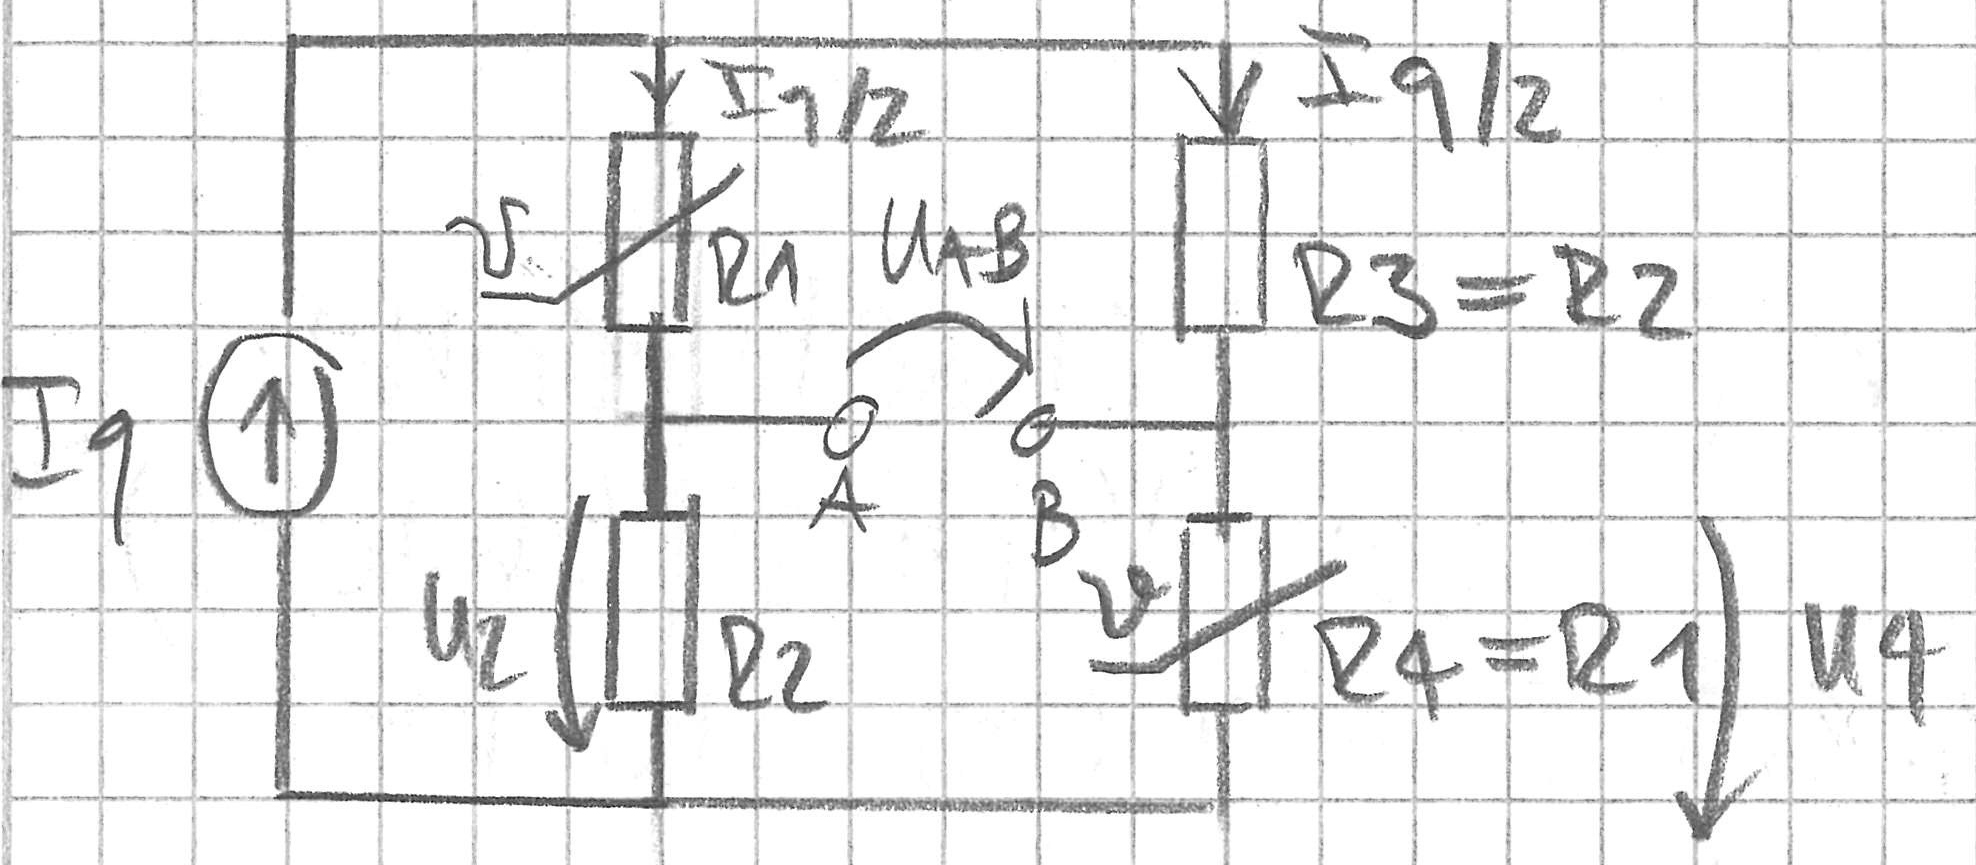
\includegraphics[width=0.3\textwidth]{pics/wheatstone/i_quelle} & 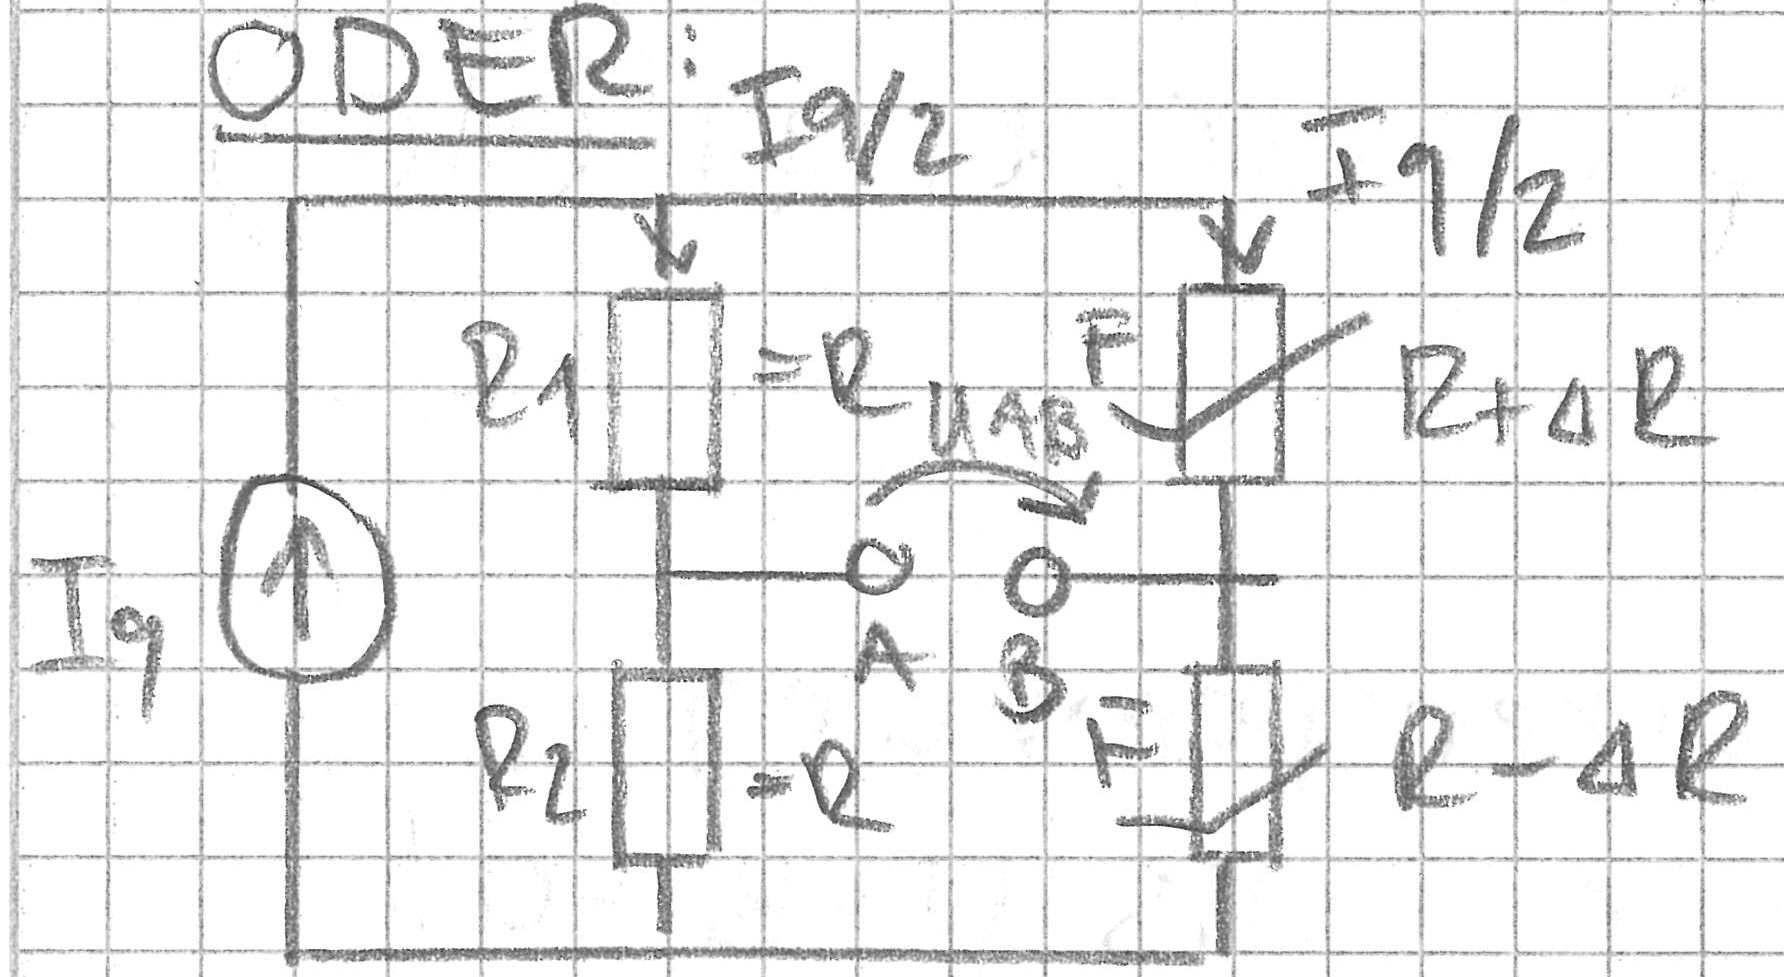
\includegraphics[width=0.25\textwidth]{pics/wheatstone/i_quelle_2}\\
$U_{AB} = U_2 - U_4$ & Ströme sind wieder gleich gross!\\
$U_{AB} = R_2 \cdot \frac{I_q}{2} - R_4 \cdot \frac{I_q}{2}$ & $U_{AB} = \frac{I_q}{2} \cdot R - \frac{I_q}{2} \cdot (R- \delta R)$\\
$U_{AB} = \frac{I_q}{2} \cdot (R_2 - R_4)$ & $U_{AB} = \frac{I_q}{2} \cdot R $\\
\end{tabular}
